\documentclass{beamer}
\usepackage[utf8]{inputenc}
\usepackage[english]{babel}
\usepackage{helvet}
\usepackage[T1]{fontenc}
\usepackage{textcomp}
\usepackage[inline]{asymptote}
\usepackage{slide_helper}
\usepackage{multirow}
\usepackage{tikz}
\usetikzlibrary{shapes.geometric, arrows}
\usepackage{pgfplots}
\pgfplotsset{compat=1.5} 
\usepgfplotslibrary{statistics}
\usetikzlibrary{external}
\tikzexternalize%

\title[MA205 - Section 2.2]{Considering Categorical Data}

\begin{document}
\begin{frame}
\titlepage
\end{frame}

\begin{frame}
\begin{example}\label{contingency table}
The following table summarizes two categorical variables from the full \dataset{loans} data set.
\begin{center}
\begin{tabular}{llcccc}
&&\multicolumn{3}{c}{\variable{homeownership}} &\\\cline{3-5}
&&\outcome{rent}&\outcome{mortgage}&\outcome{own}&Total\\\cline{2-6}
\multirow{2}{*}{{\variable{app\_type}}} & \outcome{individual} & 3496 & 3839 & 1170 & 8505 \\
&\outcome{joint} & 362 & 950 & 183 & 1495 \\\cline{2-6}
&Total & 3858 & 4789 & 1353 & 10000 \\\cline{2-6}
\end{tabular}
\end{center}
\end{example}\pause

\begin{definition}
A table that summarizes data for two categorical variables in this way is called a \textbf{contingency table}.
\end{definition}\pause

\begin{definition}
The \textbf{row totals} provide the total counts across each row.

\vspace{1mm}
The \textbf{column totals} provide the total counts down each column.
\end{definition}
\end{frame}

\begin{frame}
\begin{note}
You can also create a table that considers only a single variable.
\end{note}\pause

\begin{example}
\begin{center}
\begin{tabular}{lc}\hline
\variable{homeownership} & Count \\\hline
\outcome{rent} & 3858 \\
\outcome{mortgage} & 4789 \\
\outcome{own} & 1353 \\\hline
Total & 10000 \\\hline
\end{tabular}
\end{center}
\end{example}
\end{frame}

\begin{frame}
\begin{definition}
A \textbf{bar plot} plots a bar for each variable outcome, the height is the frequency of the outcome.
\end{definition}\pause

\begin{example}\label{bar example 1}
\begin{center}
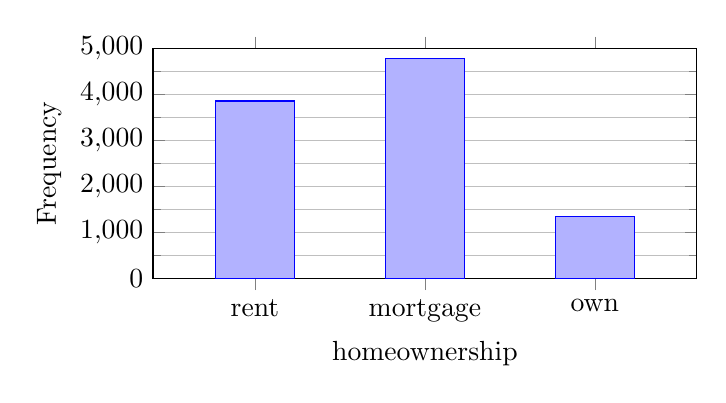
\begin{tikzpicture}
\begin{axis}[
height=4.5cm,
width=0.7\textwidth,
enlarge x limits=0.3,
ymajorgrids=true,
minor y tick num=1,
yminorgrids=true,
ylabel={Frequency},
xlabel={\variable{homeownership}},
bar width=1cm,
symbolic x coords={rent, mortgage, own},
ybar,
ymin=0,
ymax=5000,
ytick={0,1000,...,5000},
xtick=data,
xticklabel=\outcome{\tick},
]
\addplot+
coordinates
{
(rent, 3858)
(mortgage, 4789)
(own, 1353)
};
\end{axis}
\end{tikzpicture}
\end{center}
\end{example}\pause

\begin{note}
A histogram has no gaps between the bars, where as bar plot does.
\end{note}
\end{frame}

\begin{frame}
\begin{definition}
A bar plot that has been sorted so the largest bar is on the left and the smallest bar on the right is called \textbf{Pareto chart}.
\end{definition}\pause

\begin{example}
Here is the Pareto chart for the bar plot in Example~\ref{bar example 1}.
\begin{center}
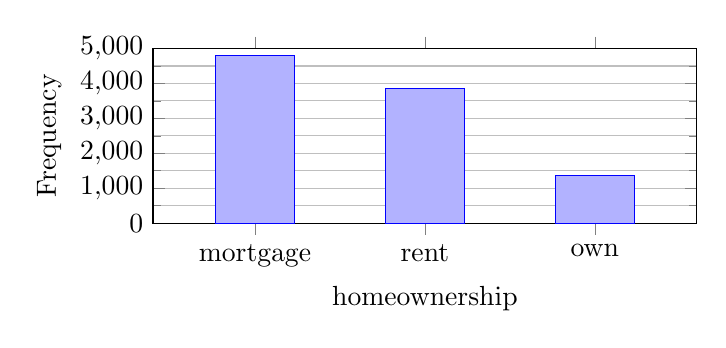
\begin{tikzpicture}
\begin{axis}[
height=3.8cm,
width=0.7\textwidth,
enlarge x limits=0.3,
ymajorgrids=true,
minor y tick num=1,
yminorgrids=true,
ylabel={Frequency},
xlabel={\variable{homeownership}},
bar width=1cm,
symbolic x coords={mortgage, rent, own},
ybar,
ymin=0,
ymax=5000,
ytick={0,1000,...,5000},
xtick=data,
xticklabel=\outcome{\tick},
]
\addplot+
coordinates
{
(mortgage, 4789)
(rent, 3858)
(own, 1353)
};
\end{axis}
\end{tikzpicture}
\end{center}
\end{example}\pause

\begin{note}
The name comes from Vilfredo Pareto, a noted Italian economist.
\end{note}
\end{frame}

\begin{frame}
\begin{note}
Instead of using frequencies, we could instead use proportions.
\end{note}\pause

\begin{example}
To find the proportion, divide each frequency by the total count.
\begin{center}
\renewcommand{\arraystretch}{2.2}
\begin{tabular}{lcc}\hline
\variable{homeownership} & Frequency & Proportion \\\hline
\outcome{rent} & 3858 & \visible<3->{$\dfrac{3858}{10000}=0.3858$} \\
\outcome{mortgage} & 4789 & \visible<4->{$\dfrac{4789}{10000}=0.4789$} \\
\outcome{own} & 1353 & \visible<5->{$\dfrac{1353}{10000}=0.1353$} \\[1mm]\hline
Total & 10000 & \visible<6->{$1.0000$} \\\hline
\end{tabular}
\end{center}
\end{example}
\end{frame}

\begin{frame}
\begin{example}
Here are both the frequency and proportion for \texttt{homeownership}.
\begin{center}
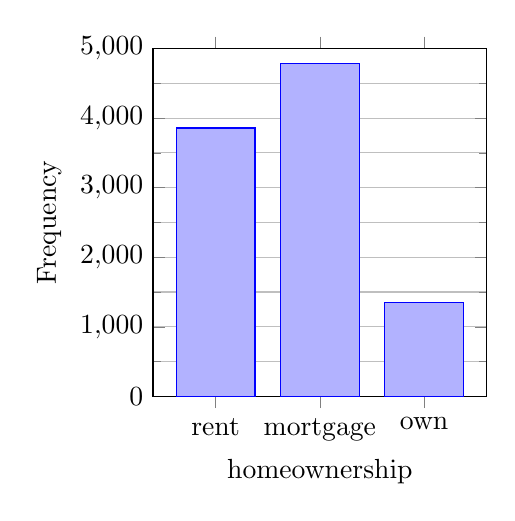
\begin{tikzpicture}
\begin{axis}[
height=6.0cm,
width=0.48\textwidth,
enlarge x limits=0.3,
ymajorgrids=true,
minor y tick num=1,
yminorgrids=true,
ylabel={Frequency},
xlabel={\variable{homeownership}},
bar width=1cm,
symbolic x coords={rent, mortgage, own},
ybar,
ymin=0,
ymax=5000,
ytick={0,1000,...,5000},
xtick=data,
xticklabel=\outcome{\tick},
]
\addplot+
coordinates
{
(rent, 3858)
(mortgage, 4789)
(own, 1353)
};
\end{axis}
\end{tikzpicture}
%
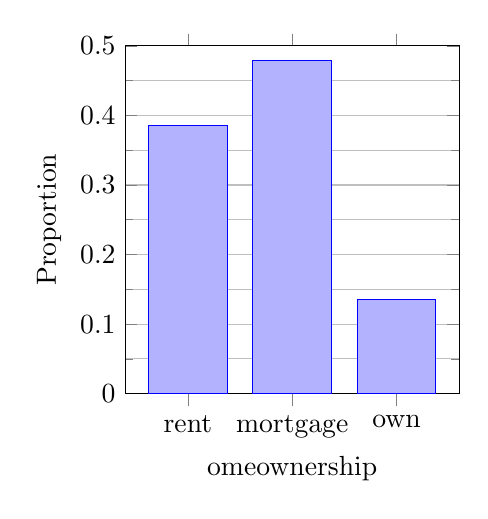
\begin{tikzpicture}
\begin{axis}[
height=6.0cm,
width=0.48\textwidth,
enlarge x limits=0.3,
ymajorgrids=true,
minor y tick num=1,
yminorgrids=true,
ylabel={Proportion},
xlabel={\variable{omeownership}},
bar width=1cm,
symbolic x coords={rent, mortgage, own},
ybar,
ymin=0,
ymax=0.5,
ytick={0,0.1,...,0.6},
xtick=data,
xticklabel=\outcome{\tick},
]
\addplot+
coordinates
{
(rent, 0.3858)
(mortgage, 0.4789)
(own, 0.1353)
};
\end{axis}
\end{tikzpicture}
\end{center}
\end{example}
\end{frame}

\begin{frame}
\begin{example}
Here, we use the \textbf{row proportions} for the contingency table from Example~\ref{contingency table}. Where we divide each count by their row total.
\begin{center}
\begin{tabular}{llcccc}
&&\multicolumn{3}{c}{\variable{homeownership}} &\\\cline{3-5}
&&\outcome{rent}&\outcome{mortgage}&\outcome{own}&Total\\\cline{2-6}
\multirow{2}{*}{{\variable{app\_type}}} & \outcome{individual} & 3496 & 3839 & 1170 & 8505 \\
&\outcome{joint} & 362 & 950 & 183 & 1495 \\\cline{2-6}
&Total & 3858 & 4789 & 1353 & 10000 \\\cline{2-6}
&&&$\downarrow~\downarrow~\downarrow$\\
&&\multicolumn{3}{c}{\variable{homeownership}} &\\\cline{3-5}
&&\outcome{rent}&\outcome{mortgage}&\outcome{own}&Total\\\cline{2-6}
\multirow{2}{*}{{\variable{app\_type}}} & \outcome{individual} & 0.4111 & 0.4514 & 0.1376 & 1.0000 \\
&\outcome{joint} & 0.2421 & 0.6355 & 0.1224 & 1.0000 \\\cline{2-6}
&Total & 0.3858 & 0.4789 & 0.1353 & 1.0000 \\\cline{2-6}
\end{tabular}
\end{center}\pause
\question{What does the number 0.4111 represent?}\pause
\answer{That $41.11\%$ of those that applied as individuals are renters.}
\end{example}
\end{frame}

\begin{frame}
\begin{example}\label{column proportion}
Here, we use the \textbf{column proportions} for the contingency table from Example~\ref{contingency table}. Where we divide each count by their column total.
\begin{center}
\begin{tabular}{llcccc}
&&\multicolumn{3}{c}{\variable{homeownership}} &\\\cline{3-5}
&&\outcome{rent}&\outcome{mortgage}&\outcome{own}&Total\\\cline{2-6}
\multirow{2}{*}{{\variable{app\_type}}} & \outcome{individual} & 3496 & 3839 & 1170 & 8505 \\
&\outcome{joint} & 362 & 950 & 183 & 1495 \\\cline{2-6}
&Total & 3858 & 4789 & 1353 & 10000 \\\cline{2-6}
&&&$\downarrow~\downarrow~\downarrow$\\
&&\multicolumn{3}{c}{\variable{homeownership}} &\\\cline{3-5}
&&\outcome{rent}&\outcome{mortgage}&\outcome{own}&Total\\\cline{2-6}
\multirow{2}{*}{{\variable{app\_type}}} & \outcome{individual} & 0.9062 & 0.8016 & 0.8647 & 0.8505 \\
&\outcome{joint} & 0.0946 & 0.1984 & 0.1353 & 0.1495 \\\cline{2-6}
&Total & 1.0000 & 1.0000 & 1.0000 & 1.0000 \\\cline{2-6}
\end{tabular}
\end{center}\pause
\question{What does the number 0.9062 represent?}\pause
\answer{That $90.62\%$ of renters applied as individuals.}
\end{example}
\end{frame}

\begin{frame}
\begin{example}
Let us look at the column proportions from Example~\ref{column proportion} more closely.
\begin{center}
\vspace{-2mm}
\begin{tabular}{llcccc}
&&\multicolumn{3}{c}{\variable{homeownership}} &\\\cline{3-5}
&&\outcome{rent}&\outcome{mortgage}&\outcome{own}&Total\\\cline{2-6}
\multirow{2}{*}{{\variable{app\_type}}} & \outcome{individual} & 0.9062 & 0.8016 & 0.8647 & 0.8505 \\
&\outcome{joint} & 0.0946 & 0.1984 & 0.1353 & 0.1495 \\\cline{2-6}
&Total & 1.0000 & 1.0000 & 1.0000 & 1.0000 \\\cline{2-6}
\end{tabular}
\end{center}\pause
Notice that 90.62\% of renters applied as individuals, which is higher than for those with mortgages (80.16\%) or those who own (86.47\%).\pause

\vspace{1mm}
Because these rates vary between the three levels of \variable{homeowndership} (\outcome{rent}, \outcome{mortgage}, \outcome{own}), there is evidence that the \variable{app\_type} and \variable{homeownsership} variables are associated.
\end{example}\pause

\begin{note}
If we had considered row proportions instead, we would look down columns to see if the fraction of loans where the borrower rents, has a mortgage, or owns varied across the \outcome{individual} to \outcome{joint} types.
\end{note}
\end{frame}
\end{document}
